Utilizando o principio de Platooning e aplicando-o ao mundo real, facilmente nos apercebemos de muitas das suas limitações. Como ponto inicial temos a restrição a uma só faixa, o que leva a que este paradigma acabe por ser aplicável praticamente apenas a veículos pesados, considerando que estes veículos mudam de faixa com relativamente menos frequência do que veículos ligeiros. No entanto considerar que platooning "tradicional" se aplica apenas em veículos pesados não é uma solução viável. Tendo em conta uma possível adopção em massa deste tipo de tecnologia, e a circulação de cada vez mais pelotões nas estradas, a utilização de apenas uma faixa tornar-se-ia inviável. Um pelotão que tenha pela frente uma viagem mais longa, ou deseje ir mais depressa, deve ter a possibilidade de poder ultrapassar pelotões mais lentos, forçando assim o uso de múltiplas faixas.

O conceito de multi-lane platooning surge então como uma possível solução para esta questão, trazendo consigo muitas mais potencialidades. Numa altura em que o tópico da condução autónoma está em voga não podemos deixar de considerar esta abordagem como uma possibilidade válida e praticável para a generalização da mesma. Implementações de multi-lane platooning no mundo real começam a ser cada vez mais plausíveis, grande parte das tecnologias necessárias já existem, quer no que toca a software quer no que toca a hardware. Resta então haver um desenho traçado de qual o rumo a seguir, quais as especificações de um sistema funcional e seguro e que infraestruturas serão necessárias para o mesmo.

\begin{figure}[H]
    \centering
    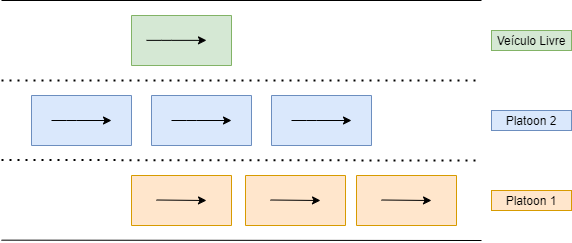
\includegraphics[scale=0.4]{Images/multilaneplatooning.png}
    \caption{Multi-Lane Platooning}
    \label{fig:my_label}
\end{figure}

Multi-lane platooning pode então ser descrito como uma aplicação/evolução do platooning tradicional a um ambiente com múltiplas faixas, prometendo uma melhoria em termos de area util das estradas, economização de combustivel e consequente redução de emissões, bem como um maior nivel de segurança. Numa implementação a médio prazo devemos também considerar a possibilidade de termos um ambiente composto por veículos mistos, considerando "misto" como sendo a representação da mistura de veículos com habilitações para integrar platoons (em termos de software/hardware) e veículos sem qualquer tipo capacidade para tal.

% Please add the following required packages to your document preamble:
% \usepackage{booktabs}
% \usepackage{graphicx}
\begin{table}[H]
\resizebox{\textwidth}{!}{%
\begin{tabular}{@{}ll@{}}
\toprule
\textbf{Platooning Tradicional}  & \textbf{Multi-lane Platooning}         \\ \midrule
Faz uso de uma só via            & Faz uso de várias vias                 \\ \midrule
Não otimizado ao espaço útil     & Otimizado ao espaço útil               \\ \midrule
Mais adequado a veículos pesados & Adequado a veículos ligeiros e pesados \\ \midrule
Implementação menos complexa     & Implementação mais complexa            \\ \midrule
Geralmente não necessita de infraestruturas externas & Infraestruturas externas são comumente sugeridas \\ \bottomrule
\end{tabular}%
}
\caption{Platooning vs Multi-lane Platooning}
\label{tab:my-table}
\end{table}



Cada platoon formado, para além da condução autónoma deve assumir alguns comportamentos de grupo de forma a garantir um funcionamento do grupo como um todo. Um platoon, de modo geral, precisa de ser liderado, quer por um elemento do mesmo (uma liderança centralizada no platoon) quer por um sistema de controlo externo (uma liderança descentralizada). Uma liderança descentralizada pode ter um custo inicial maior, considerando que o sistema responsável por coordenar tanto os platoons como os veículos tem que ser desenvolvido, bem como infraestruturas que suportem o mesmo, no entanto, em teoria, confere uma maior escalabilidade.

Para além da questão da liderança os veículos integrantes do pelotão devem se capazes de seguir certas regras dentro do mesmo. Estes devem ser capaz de manter uma distância uniforme, ajustando a mesma segundo as condições climatéricas que se façam sentir [Artigo3 ??]. Estes veículos devem ser também capazes de responder em conjunto a eventos não previstos, seja exemplo uma travagem de emergência.

\begin{figure}[H]
    \centering
    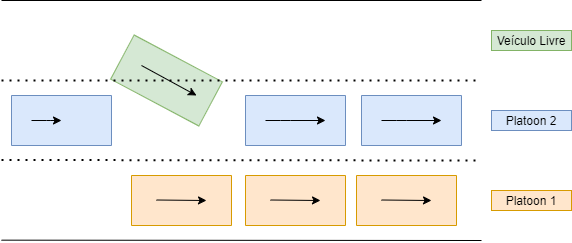
\includegraphics[scale=0.4]{Images/brakeCheck.png}
    \caption{Travagem de emergência}
    \label{fig:my_label}
\end{figure}
\begin{center}
    Após a travagem iniciada todo os veículos que seguem atrás do veiculo que iniciou a travagem devem também ser capazes de reduzir a velocidade de forma a evitar qualquer tipo de contacto entre eles
\end{center}

Ainda dentro dos comportamentos sociais dentro dos pelotões temos o processo de Merge e Split, processos pelos quais veículos se juntam e abandonam o pelotão (respectivamente). A forma mais simples de um veículo se juntar a um pelotão consiste em juntar-se ao fundo da fila, no entanto se o mesmo não for possível o veículo deverá ter a possibilidade de entrar noutra zona do pelotão, mediante comunicação com os veículos integrantes. Algumas implementações na literatura [Referências] sugerem que esta manobra pode ser feita de forma não autónoma pelo condutor do veículo, no entanto numa implementação ideal julgamos que o processo deva ser completamente autónomo. O processo de Split é inerentemente mais fácil, consistindo num "abandono" de um pelotão por parte de um veículo. Após a saida do mesmo os veículos que seguiam atrás do veículo \textit{Splitter} devem reduzir o espaçamento para o veículo seguinte, cobrindo o espaço deixado pelo veículo que abandona a fila.

\begin{figure}[H]
    \centering
    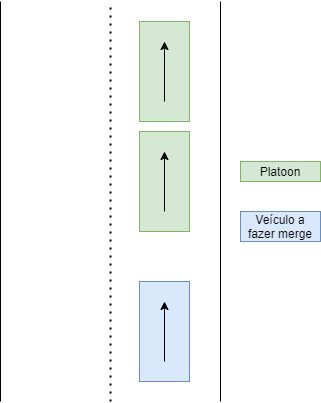
\includegraphics[scale=0.4]{Images/Merge.png}
    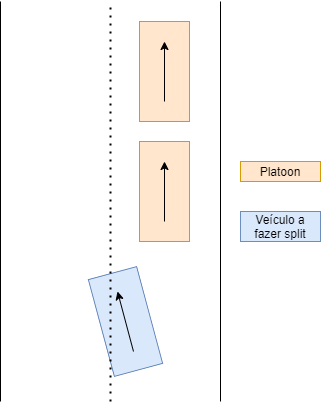
\includegraphics[scale=0.4]{Images/Split.png}
    \caption{Merge (esquerda) e Split (direita)}
    \label{fig:my_label}
\end{figure}

Num sistema com múltiplas faixas um ponto importante do comportamento de grupo dos pelotões prende-se com a alteração de faixa. Em 2007 Dao, Clark e Huissoon discutiam este assunto, como se pode ler em \cite{cite10,citeE4}.

O processo de decisão responsável por definir que faixa um veículo, ou, no nosso caso, um pelotão deles, vai assumir deve considerar a capacidade máxima de cada faixa, e o quão próximo do limite de veículos cada faixa está. O plano de atribuição de faixas aos veículos presentes na zona em questão deve ser feito tendo em conta todos os veículos (ou pelotões). Este processo de decisão poderá ser feito entre os pelotões (ou entre os seus lideres) no caso de ser um sistema centralizado (veículos/pelotões tomam as suas próprias decisões) ou por um sistema descentralizado responsável por "controlar" os veículos e as suas ações. 
